\section{Migovec's Long Term Prospects}


\begin{marginfigure}
\checkoddpage \ifoddpage \forcerectofloat \else \forceversofloat \fi
\centering
 \frame{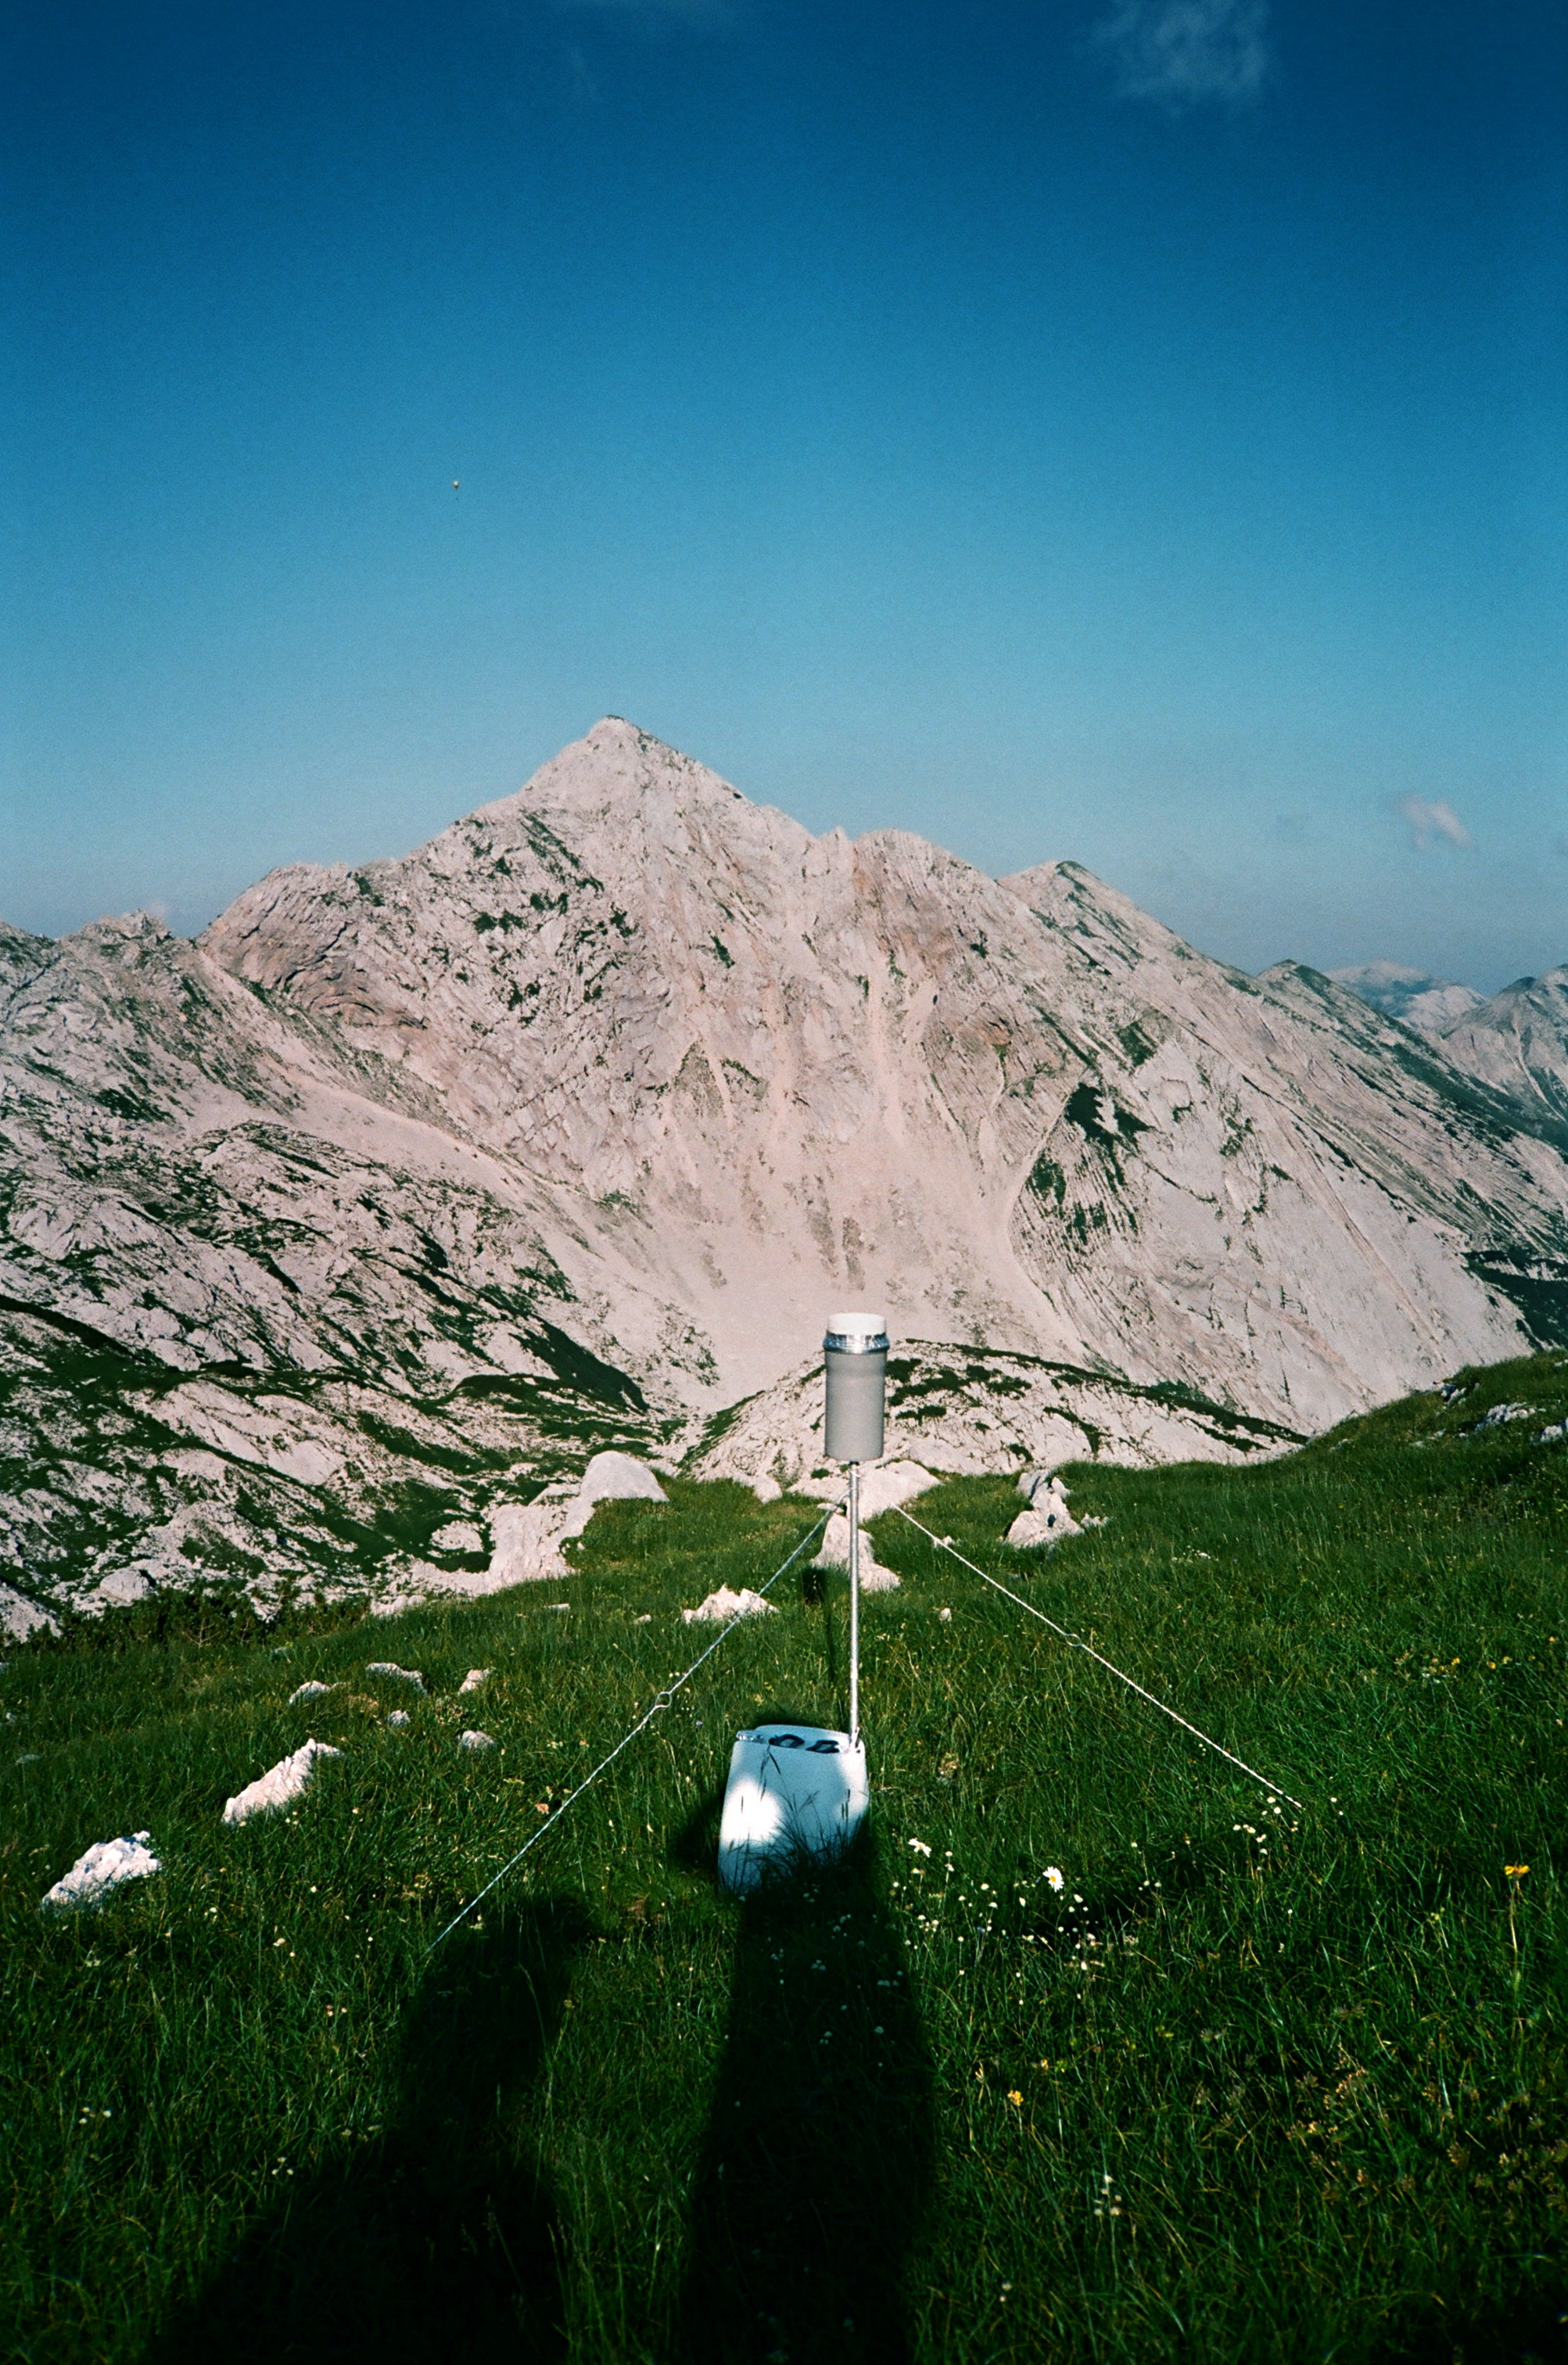
\includegraphics[width=\linewidth]{2010/outlook/jarvist frost - olympus xa - superia 100 - 2009 - rain gauge with skrbina in background--orig.jpg}} 
 \caption{A rain gauge with an enviable view of \passage[mountain]{Migovec}'s neighbouring mountain \passage[mountain]{Vrh nad Škrbino}. \pic{Jarvist Frost}}
 \label{rain gauge}
\end{marginfigure}

It has been a recurrent discussion in our club as to when we will run
out of new cave to discover in \passage[mountain]{Migovec}. Almost all of our fruitful
exploration has taken place within a single square kilometre of the flat
topped mountain.

\passage[mountain]{Migovec}, being part of a mountain chain that is the first high altitude
interruption to moist air from the Adriatic, receives an extremely
significant level of rainfall. This summer, Jaka Ortar, a Slovenian
geographer, recorded 210 cm of rain on \passage[mountain]{Migovec} in 100 days (28\(^{th}\)
July-3\(^{rd}\) November) with his network of rain gauges. However we
have never found any large rivers underground --- the known cave can
only account for a tiny percentage of the total drainage for the
plateau.

Our current hypothesis is that there is no \textit{master system}
gathering the water, but instead a complex hydrology induced by cave
passage intersecting the underlying (as yet, unvisited) band of
Cretaceous shales.

For all \passage{Vrtnarija}'s complexity, the entire cave can be fitted
into a slab of limestone slanted at 66 degrees and just
\(1000\times150\times1000\) m.

Certainly, as long as we can continue to find entrances through the
frost shattered and heavily cratered surface, there will be enough cave
in \passage[mountain]{Migovec} for decades more of exploration.


\subsection{Exploration Outlook}

The significant discoveries of this year have been the fruit of the communal effort of ICCC and JSPDT members. When System \passage{Vrtnarija} and \passage{SysMig} will be connected, the cave will only be 500 m shorter than the \passage{Postonjska Jama}
system. Suddenly the plain dwellers will have to rewrite their tourist brochures and the thought of the longest cave in Slovenia
will not be a dream. Oh, and the cave has the potential to be 1km deep (requiring an additional 120 m of depth from \passage{Insomnia}).

\tweet{3:21PM Aug 15, 2010}{Van returned, all safe and sound, gear unpacked into the familiar dusty cramped confines of stores. Plans already fermenting for 2011! Out.}

As well as being proud of each metre of survey we should also think about each metre that a tackle sack was carried, each meal cooked, each bottle of booze safely ferried to camp. A significant factor in our success is evident because it needs not mentioning: thanks to efficient and thoughtful organization we did not run out of any goods, the stereo batteries were always full, the food supplies always high. And most importantly, we have no accidents to report.
